\ifnum \Version=1
\question[6] % 
Consider the differential equation $\displaystyle \dydt = (y-1)(y-2)^2$, where $y$ is a real function of $t$, and $t \ge 0$. 
\begin{parts}
    \part Draw the phase line, and determine whether the critical points (if any) are stable, semi-stable, or unstable. Please show your work. 
    \vspace{8cm}
    \part Using results from part (b) to sketch several solution curves in the $ty$-plane for $t \ge 0$. Don't forget to label your axes. 
\end{parts}

\ifnum \Solutions=1 {\color{DarkGreen} 
\textbf{Solutions:} phase line: 
\begin{center}
    \begin{tikzpicture}[ultra thick]
    \DrawHorizontalPhaseLine[$y$]{$k$,2}{5}{-1,2}%
\end{tikzpicture}
\end{center}

The critical points are:
\begin{itemize}
    \item $y=0$ which is semi-stable
    \item $y=4$ which is unstable
\end{itemize}

} 
\else 
\newpage
\fi


\fi

\ifnum \Version=2
\question[8] % 
Consider the differential equation $\displaystyle \dydt = (y-1)(y^2-4)$, where $y$ is a real function of $t$, and $t \ge 0$.
\begin{parts}
    \part Draw the phase line, and determine whether the critical points (if any) are stable, semi-stable, or unstable. Please show your work. 
    \vspace{10cm}
    \part Use results from part (a) to sketch several solution curves in the $ty$-plane for $t \ge 0$. Don't forget to label your axes. 
\end{parts}
\fi
\ifnum \Version=3
\question[8] % 
Consider the differential equation $\displaystyle \dydt = (y-2)(y-3)^2$, where $y$ is a real function of $t$, and $t \ge 0$.
\begin{parts}
    \part Draw the phase line, and determine whether the critical points (if any) are stable, semi-stable, or unstable. Please show your work. 
    \vspace{10cm}
    \part Use results from part (a) to sketch several solution curves in the $ty$-plane for $t \ge 0$. Don't forget to label your axes. 
\end{parts}
\fi 
\ifnum \Version=4
\question[8] % 
Consider the differential equation $\displaystyle \dydt = (y-1)^2(y-4)$, where $y$ is a real function of $t$, and $t \ge 0$.
\begin{parts}
    \part Draw the phase line, and determine whether the critical points (if any) are stable, semi-stable, or unstable. Please show your work. 
    \vspace{10cm}
    \part Use results from part (a) to sketch several solution curves in the $ty$-plane for $t \ge 0$. Don't forget to label your axes. 
\end{parts}
\fi 
\ifnum \Version=5
\question[8] % 
Consider the differential equation $\displaystyle \dydt = (y-1)(y^2-9)$, where $y$ is a real function of $t$, and $t \ge 0$.
\begin{parts}
    \part Draw the phase line, and determine whether the critical points (if any) are stable, semi-stable, or unstable. Please show your work. 
    \vspace{10cm}
    \part Use results from part (a) to sketch several solution curves in the $ty$-plane for $t \ge 0$. Don't forget to label your axes. 
\end{parts}
\fi  


\ifnum \Version=6
\question[4] % 
Consider the differential equation $\displaystyle \dydt = y^2(y-4)$, where $y$ is a real function of $t$, and $t \ge 0$.
\begin{parts}
    \part Draw the phase line, and determine whether the critical points (if any) are stable, semi-stable, or unstable. Please show your work. 
        \ifnum \Solutions=0 \vspace{8cm} \fi
    \part Use results from part (a) to sketch several solution curves in the $ty$-plane for $t \ge 0$. Don't forget to label your axes. 
\end{parts}

\ifnum \Solutions=1 {\color{DarkGreen} 
    \textbf{Solutions:} if we sketch the phase line we obtain the following.
    
    \begin{center}
        \begin{tikzpicture}[ultra thick]
        \DrawHorizontalPhaseLine[$y$]{0,4}{5}{-1,2}%
    \end{tikzpicture}
    \end{center}
    
    The critical points are:
    \begin{itemize}
        \item $y=0$ which is semi-stable
        \item $y=4$ which is unstable
    \end{itemize}
    Solution curves shown below. 
       \begin{center}     
    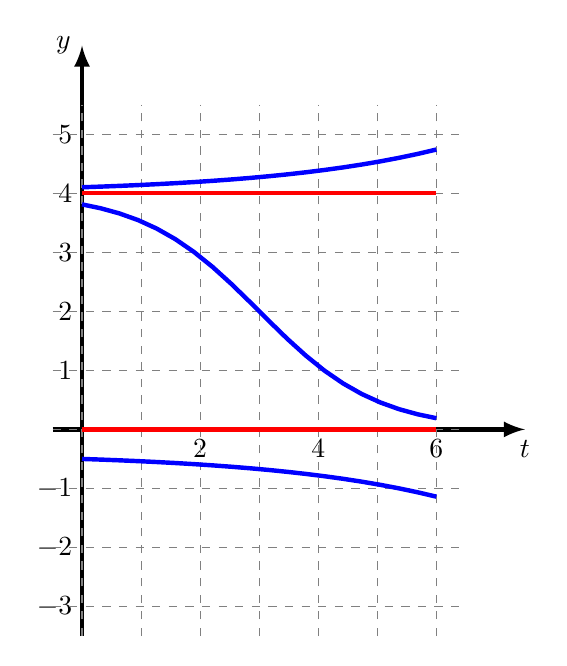
\begin{tikzpicture}[scale=0.75]
      \draw[ultra thick,->,>=latex] (-0.5,0)--(7.5,0) node[below] {$t$};
      \draw[ultra thick,->,>=latex] (0,-3.5)--(0,6.5) node[left] {$y$};
      \draw (0,1) node[left] {$1$};  
      \draw (0,2) node[left] {$2$};  
      \draw (0,3) node[left] {$3$}; 
      \draw (0,4) node[left] {$4$}; 
      \draw (0,5) node[left] {$5$}; 
      \draw (0,-1) node[left] {$-1$};  
      \draw (0,-2) node[left] {$-2$};  
      \draw (0,-3) node[left] {$-3$};       
      \draw (2,0) node[below] {$2$};          
      \draw (4,0) node[below] {$4$};          
      \draw (6,0) node[below] {$6$};          
      \draw[help lines,gray,thin,dashed] (-.5, -3.5) grid (6.5, 5.5);
      \draw[domain=0:6,ultra thick,samples=4,red] plot ({\x},{0});
      \draw[domain=0:6,ultra thick,samples=4,red] plot ({\x},{4});
      \draw[domain=0:6,ultra thick,samples=20,blue] plot ({\x},{-.4 - 0.1*exp(\x/3});
      \draw[domain=0:6,ultra thick,samples=20,blue] plot ({\x},{4+0.1*exp(\x/3});
      \draw[domain=0:6,ultra thick,samples=20,blue] plot ({\x},{4-4*(1/(1+exp(-(\x-3))))});
    \end{tikzpicture}
    \end{center}        
    
} 
\else 
\fi\fi 


\ifnum \Version=7
\question[4] % 
Consider the differential equation $\displaystyle \dydt = (y+2)(y-1)(y-3)$, where $y$ is a real function of $t$, and $t \ge 0$.
\begin{parts}
    \part Draw the phase line, and determine whether the critical points (if any) are stable, semi-stable, or unstable. Please show your work. 
    \ifnum \Solutions=0 \vspace{8cm} \fi
    \part Use results from part (a) to sketch several solution curves in the $ty$-plane for $t \ge 0$. Don't forget to label your axes. 
\end{parts}

\ifnum \Solutions=1 {\color{DarkGreen} 
    \textbf{Solutions:} if we sketch the phase line we obtain the following.
    
    \begin{center}
        \begin{tikzpicture}[ultra thick]
        \DrawHorizontalPhaseLine[$y$]{-2,1,3}{-0.5,4}{-3,2}%
    \end{tikzpicture}
    \end{center}
    
    The critical points are:
    \begin{itemize}
        \item $y=1$ stable
        \item $y=-2,3$ unstable
    \end{itemize}
    Solution curves shown below. 
    \begin{center}     
    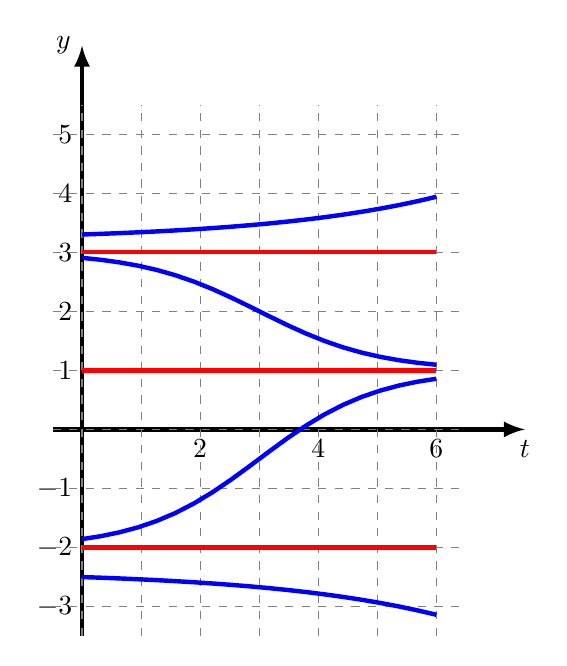
\begin{tikzpicture}[scale=0.75]
      \draw[ultra thick,->,>=latex] (-0.5,0)--(7.5,0) node[below] {$t$};
      \draw[ultra thick,->,>=latex] (0,-3.5)--(0,6.5) node[left] {$y$};
      \draw (0,1) node[left] {$1$};  
      \draw (0,2) node[left] {$2$};  
      \draw (0,3) node[left] {$3$}; 
      \draw (0,4) node[left] {$4$}; 
      \draw (0,5) node[left] {$5$}; 
      \draw (0,-1) node[left] {$-1$};  
      \draw (0,-2) node[left] {$-2$};  
      \draw (0,-3) node[left] {$-3$};       
      \draw (2,0) node[below] {$2$};          
      \draw (4,0) node[below] {$4$};          
      \draw (6,0) node[below] {$6$};          
      \draw[help lines,gray,thin,dashed] (-.5, -3.5) grid (6.5, 5.5);
      \draw[domain=0:6,ultra thick,samples=4,red] plot ({\x},{-2});
      \draw[domain=0:6,ultra thick,samples=4,red] plot ({\x},{1});
      \draw[domain=0:6,ultra thick,samples=4,red] plot ({\x},{3});
      \draw[domain=0:6,ultra thick,samples=20,blue] plot ({\x},{-2.4 - 0.1*exp(\x/3});
      \draw[domain=0:6,ultra thick,samples=20,blue] plot ({\x},{3.2+0.1*exp(\x/3});
      \draw[domain=0:6,ultra thick,samples=20,blue] plot ({\x},{3-2*(1/(1+exp(-(\x-3))))});
      \draw[domain=0:6,ultra thick,samples=20,blue] plot ({\x},{-2+3*(1/(1+exp(-(\x-3))))});
    \end{tikzpicture}
    \end{center}        
    
} 
\else 
\fi\fi 





\ifnum \Version=9
\question[4] % 
Consider the differential equation $\displaystyle \dydt = (1+y)(2-y)(4-y)$, where $y$ is a real function of $t$, and $t \ge 0$.
\begin{parts}
    \part Draw the phase line, and determine whether the critical points (if any) are stable, semi-stable, or unstable. Please show your work. 
    \ifnum \Solutions=0 \vspace{8cm} \fi
    \part Use results from part (a) to sketch several solution curves in the $ty$-plane for $t \ge 0$. Don't forget to label your axes. 
\end{parts}

\ifnum \Solutions=1 {\color{DarkGreen} 
    \textbf{Solutions:} if we sketch the phase line we obtain the following.
    
    \begin{center}
        \begin{tikzpicture}[ultra thick]
        \DrawHorizontalPhaseLine[$y$]{-1,2,4}{0.5,5}{-2,3}%
    \end{tikzpicture}
    \end{center}
    
    The critical points are:
    \begin{itemize}
        \item $y=1$ stable
        \item $y=-2,3$ unstable
    \end{itemize}
    Solution curves shown below. 
    \begin{center}     
    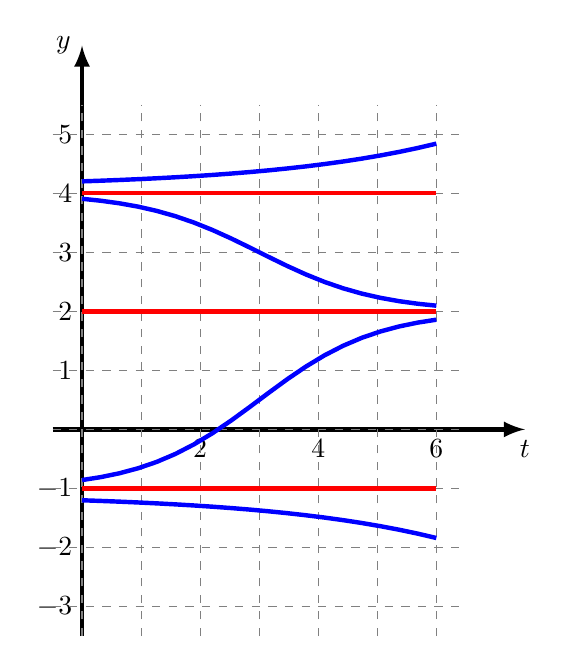
\begin{tikzpicture}[scale=0.75]
      \draw[ultra thick,->,>=latex] (-0.5,0)--(7.5,0) node[below] {$t$};
      \draw[ultra thick,->,>=latex] (0,-3.5)--(0,6.5) node[left] {$y$};
      \draw (0,1) node[left] {$1$};  
      \draw (0,2) node[left] {$2$};  
      \draw (0,3) node[left] {$3$}; 
      \draw (0,4) node[left] {$4$}; 
      \draw (0,5) node[left] {$5$}; 
      \draw (0,-1) node[left] {$-1$};  
      \draw (0,-2) node[left] {$-2$};  
      \draw (0,-3) node[left] {$-3$};       
      \draw (2,0) node[below] {$2$};          
      \draw (4,0) node[below] {$4$};          
      \draw (6,0) node[below] {$6$};          
      \draw[help lines,gray,thin,dashed] (-.5, -3.5) grid (6.5, 5.5);
      \draw[domain=0:6,ultra thick,samples=4,red] plot ({\x},{-1});
      \draw[domain=0:6,ultra thick,samples=4,red] plot ({\x},{2});
      \draw[domain=0:6,ultra thick,samples=4,red] plot ({\x},{4});
      \draw[domain=0:6,ultra thick,samples=20,blue] plot ({\x},{-1.1 - 0.1*exp(\x/3});
      \draw[domain=0:6,ultra thick,samples=20,blue] plot ({\x},{4.1+0.1*exp(\x/3});
      \draw[domain=0:6,ultra thick,samples=20,blue] plot ({\x},{4-2*(1/(1+exp(-(\x-3))))});
      \draw[domain=0:6,ultra thick,samples=20,blue] plot ({\x},{-1+3*(1/(1+exp(-(\x-3))))});
    \end{tikzpicture}
    \end{center}        
    
} 
\else 
\fi\fi 



\ifnum \Version=8
\question[4] % 
Consider the differential equation $\displaystyle \dydt = (y+2)(y-2)^2$, where $y$ is a real function of $t$, and $t \ge 0$.
\begin{parts}
    \part Draw the phase line, and determine whether the critical points (if any) are stable, semi-stable, or unstable. Please show your work. 
        \ifnum \Solutions=0 \vspace{8cm} \fi
    \part Use results from part (a) to sketch several solution curves in the $ty$-plane for $t \ge 0$. Don't forget to label your axes. 
\end{parts}

\ifnum \Solutions=1 {\color{DarkGreen} 
    \textbf{Solutions:} if we sketch the phase line we obtain the following.
    
    \begin{center}
        \begin{tikzpicture}[ultra thick]
        \DrawHorizontalPhaseLine[$y$]{-2,2}{0,3}{-3}%
    \end{tikzpicture}
    \end{center}
    
    The critical points are:
    \begin{itemize}
        \item $y=2$ which is semi-stable
        \item $y=-2$ which is unstable
    \end{itemize}
    Solution curves shown below. 
       \begin{center}     
    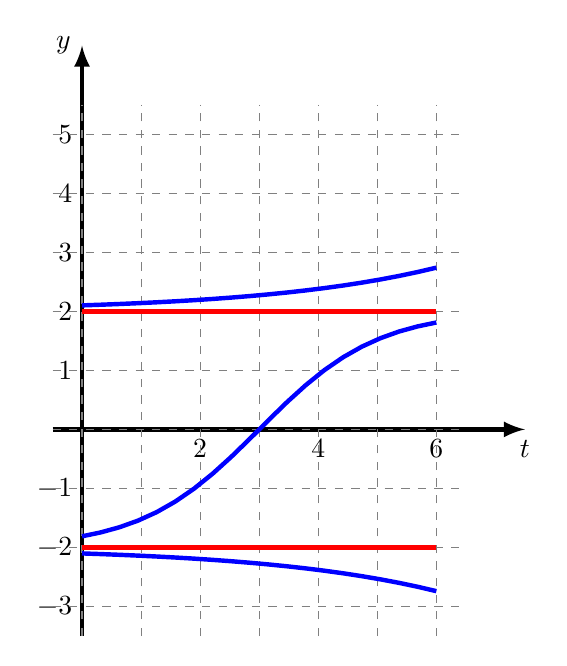
\begin{tikzpicture}[scale=0.75]
      \draw[ultra thick,->,>=latex] (-0.5,0)--(7.5,0) node[below] {$t$};
      \draw[ultra thick,->,>=latex] (0,-3.5)--(0,6.5) node[left] {$y$};
      \draw (0,1) node[left] {$1$};  
      \draw (0,2) node[left] {$2$};  
      \draw (0,3) node[left] {$3$}; 
      \draw (0,4) node[left] {$4$}; 
      \draw (0,5) node[left] {$5$}; 
      \draw (0,-1) node[left] {$-1$};  
      \draw (0,-2) node[left] {$-2$};  
      \draw (0,-3) node[left] {$-3$};       
      \draw (2,0) node[below] {$2$};          
      \draw (4,0) node[below] {$4$};          
      \draw (6,0) node[below] {$6$};          
      \draw[help lines,gray,thin,dashed] (-.5, -3.5) grid (6.5, 5.5);
      \draw[domain=0:6,ultra thick,samples=4,red] plot ({\x},{-2});
      \draw[domain=0:6,ultra thick,samples=4,red] plot ({\x},{2});
      \draw[domain=0:6,ultra thick,samples=20,blue] plot ({\x},{-2-0.1*exp(\x/3});
      \draw[domain=0:6,ultra thick,samples=20,blue] plot ({\x},{2+0.1*exp(\x/3});
      \draw[domain=0:6,ultra thick,samples=20,blue] plot ({\x},{-2+4*(1/(1+exp(-(\x-3))))});
    \end{tikzpicture}
    \end{center}        
    
} 
\else 
\fi\fi 